\section{Båndpassfilter}\label{sec:filter}
Til at fjerne støj og andre udefrakommende forstyrrelser i systemet, skal der laves et filter.
Der vil her blive designet et aktivt båndpas filter, da der kun ønskes at én bestemt frekvens forstærkes.
Fordelen ved det aktive filter er at den kan både forstærke og filtrere.

\subsection{Design}
Den valgte opstilling der anvendes er taget fra figur 5.1-4 \cite[side. 208]{Huelsman1993}.
\husk{Nikolaj}{Indsæt schematic af det aktive filter fra bogen}
Filteret er designet så modstanden $R_5$ gør forstærkningen ved centerfrekvens til en fri variable.
Heraf designes filteret efter en ønsket båndbredde, centerfrekvens og centerfrekvens forstærkning. Q er systemets godhed og anvendes til at bestemme bredden på båndbredden. 
$\omega_c$ er centerfrekvensen der bestemmer ved hvilken frekvens filterets maksimale forstærkning optræde.
$H_o$ er forstærkningen ved den ønskede centerfrekvens.
\subsection{Beregninger}
Filteret har varierende forstærkning ved forskellige frekvenser hvori centerfrekvensen har den største forstærkning. For at udregne modstandsværdier skal der vælges størrelse på kondensatorene, forstærkning ved centerfrekvens og filterets godhed.
Det er her besluttet at begge kondensatorer skal være lige store for at simplificerer udregningerne.
Kondensatoren vælges til $C_{10} = 470 \si{\pico\farad}$, godheden vælges til $Q = 3$, centerfrekvens forstærkingen vælges til $H_o = 3$ og centerfrekvensen vælges til $F_c = 46.936 \si{\kilo\ohm}$.
Heraf udregnes båndbredden for filteret og filtermodstandene \cite[Side. 209]{Huelsman1993}.
Til udregning af centervinkelfrekvensen henvises til ligning \ref{eq:vinkelfrekvens}.
\begin{align}
	B & = \frac{F_c}{Q}
	\end{align}
Filterets båndbredde er givet ved forholdet mellem centerfrekvensen og filterets godhed, båndbredden kan også gøre systemet hurtigere hvis den er bred.
\begin{align}
	R_8 & = \frac{Q}{\omega_c \cdot C_{filter} \cdot H_o } \label{eq:R8}
	\end{align}
Filterets indgangsmodstand er med til at påvirke systemets centerfrekvens forstærkning, men den kan ikke alene gøre den til en fri variable. 
\begin{align}
	R_9 & = \frac{Q}{ \omega_c \cdot C_{filter} \cdot \left( 2 \cdot Q^2 - H_o \right) } \label{eq:R9}
	\end{align}
Modstanden $R_9$ er med til at gøre forstærkningen til en fri variabel, hvis denne ikke var med så havde filterets forstærkning været afhængig af godheden.
\begin{align}
	R_{10} & = \frac{2 \cdot Q}{ \omega_c \cdot C} \label{eq:R10}
\end{align}
Feedback modstanden regnes ved ligning \ref{eq:R10}.
Dette medfører. $R_8 = 7.215 \si{\kilo\ohm}$, $R_9 = 1.430 \si{\kilo\ohm}$, $R_{10} = 43.288 \si{\kilo\ohm}$ og $B = 15.645 \si{\kilo\ohm}$.
Da disse modstands værdier ikke kan realiseres i SMD, vælges derfor tilnærmede størrelser.
De tilnærmede komponentværdier kommer til at være. $R_8 = 6.8 \si{\kilo\ohm}$, $R_9 = 1.5 \si{_\kilo\ohm}$ og $R_{10} = 47 \si{\kilo\ohm}$.
De tilpassede komponenter medfører at systemet har en anden karakteristik end den udregnede. 
Til udregning anvendes ligningerne 13a, 13b og 13c \cite[Side. 208]{Huelsman1993}. 
\begin{align}
	F_c & = \frac{\sqrt{1+\frac{R_9}{R_8}}}{\left( 2 \cdot \pi \right) \cdot \sqrt{R_9 \cdot R_{10} \cdot C_{10}^2}}
	\end{align}
Centerfrekvensen ændrer sig hvis de teoretiske værdier ikke kan opfyldes. Denne ligning bruges til at udregne hvor den nye centerfrekvens kommer til at ligge.
\begin{align}
	Q & = \left( \frac{2 \cdot \sqrt{\frac{R_9 \cdot C_{10}}{R_{10} \cdot C_{10}}}}{\sqrt{1+\frac{R_9}{R_8}}} \right)^{-1}
	\end{align}
Når kondensatorene er lige store så har de ingen indflydelse på filterets godhed. Denne ligning er kun afhængig af modstandsværdierne i dette tilfælde.
\begin{align}
	H_o & = \frac{\frac{R_{10}}{R_8}}{1+\frac{C_{10}}{C_{10}}}
\end{align}
Tilsvarende for godheden så har kondensatorene ikke nogen påvirkning når de er lige store.
Ændringen er her udelukkende afhængig af indgangs og feedback modstand.
Dette medfører at systemets karakteristik er. 
$H_o = 3.5$, $F_c = 44.557 \si{\kilo\hertz}$, $Q = 3.1$ og $B = 14.4 \si{\kilo\hertz}$. 
En forøgelse på $16 \%$ på forstærkningen kommer ikke til at blive et problem så længe instrumenterings forstærkeren ikke går i mætning. 
Centerfrekvens ændringen er acceptabel da den ikke ligger så langt fra den teoretiske at det forårsager den dæmpning af spændingen.
En højere godhed medfører at at båndbredden bliver mindre, men da båndbredden stadig er stor så kommer det ikke til at gøre systemet signifikant langsommere.

\begin{figure}[h!]
	\centering
	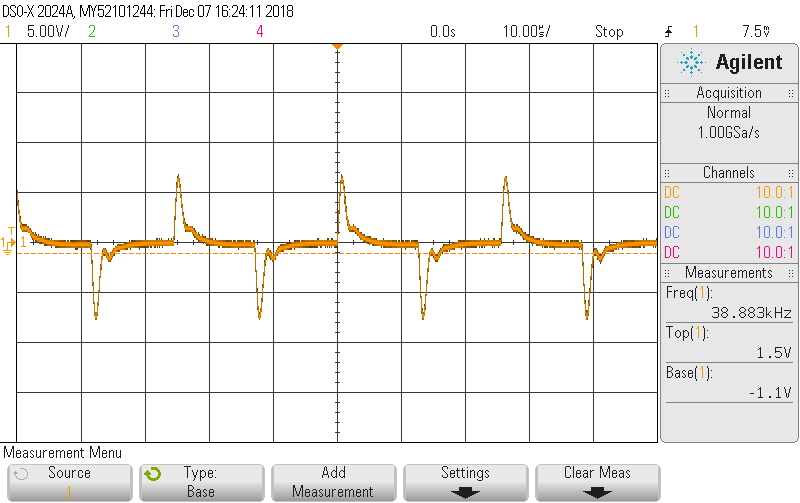
\includegraphics[width=1\textwidth]{billeder/filter_in_png.png}
	\caption{Her ses signalet fra modtagerspolen før filteret.}
	\label{fig:filter_in}
\end{figure}

\begin{figure}[h!]
	\centering
	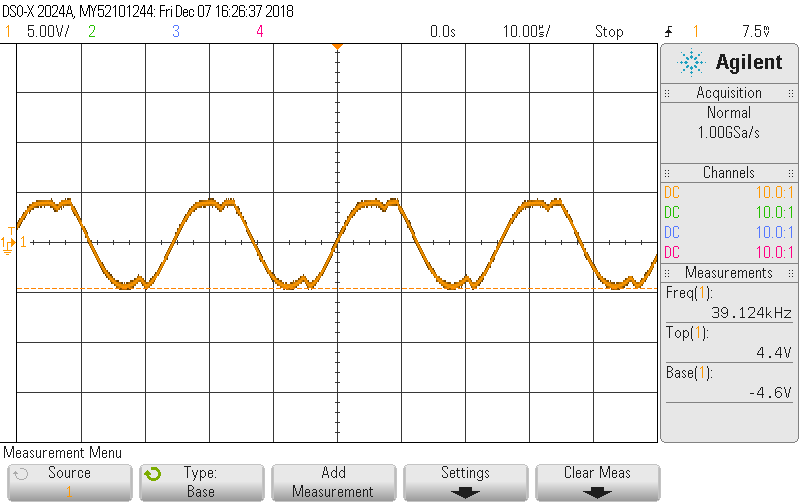
\includegraphics[width=1\textwidth]{billeder/filter_out_png.png}
	\caption{Her ses signalet efter filteret, hvor signalet er forstærket i filteret.}
	\label{fig:filter_out}
\end{figure}